\documentclass[12pt]{article}
\usepackage{amsfonts}
\usepackage{amsmath}
\usepackage{graphicx} 
\usepackage{float}
\usepackage[caption = false]{subfig}
\usepackage{/Users/timbarry/Documents/optionFiles/mymacros}

\title{Machine hypothesis testing in multi-axis, high-throughput data}
\author{Tim B}
\begin{document}
\maketitle
\section{The explosion of multi-axis high-throughput data}

A transformation occurred in statistics at the turn of the twentieth century. New biotechnologies, including as microarrays, GWAS, and bulk RNA-seq, yielded tens of thousands (or more) of measurements, necessitating the development of new statistical approaches to handling many hypotheses (e.g., FDR; Figure \ref{fig:technologies}). These technologies yielded many measurements along a \textit{single} axis (Figure \ref{fig:calibration_sets}b-c). For example, in microarrays and bulk RNA-seq, expression level is measured for many genes ($Y_1, \dots, Y_p$) across an experimental condition (e.g., diseased or healthy). In this sense microarray and bulk RNA-seq data are ``wide.'' By contrast, in GWAS, many genetic variants $(X_1, \dots, X_d)$ are measured, their their association with a phenotype is tested. In this sense GWAS data are ``tall.'' (Note that ``tall'' and ``wide'' here refer to the number of features measured along different axes of the data, not the dimension of the data. Whether a dataset is ``tall'' or ``wide'' in this context is orthogonal to whether it is low- or high-dimensional.) We note that scientists sometimes conduct multi-trait GWAS studies, but these studies are ``low throughput'' in the number of traits (i.e., a few traits, rather than tens or hundreds of thousands of traits, are examined). 

\begin{figure}[h!]
	\centering
	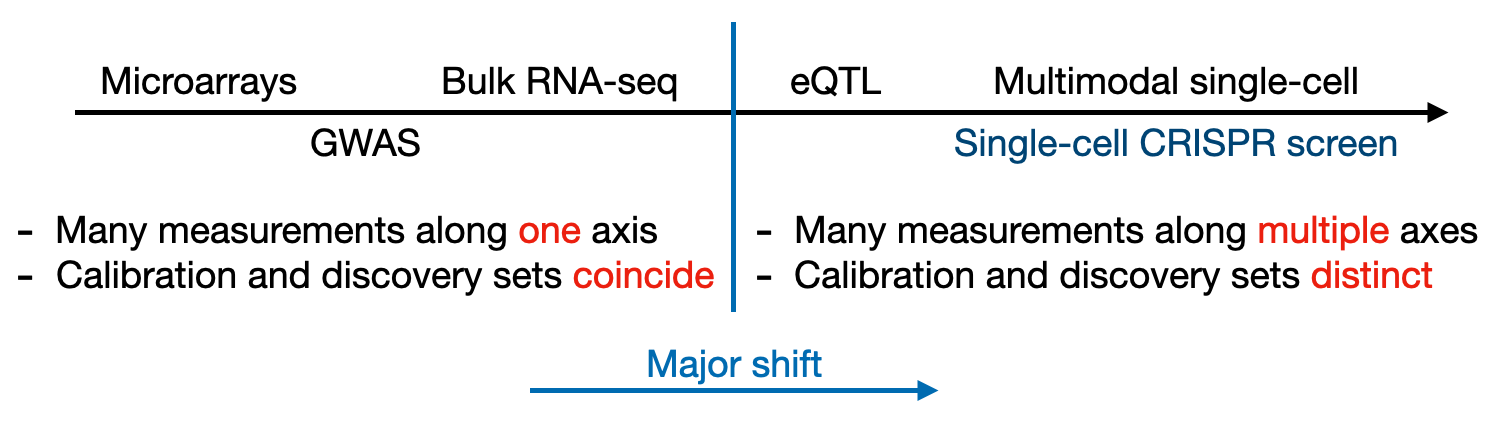
\includegraphics[width=1\linewidth]{technologies}
	\caption{Older technologies (e.g., microarrays, GWAS, and bulk RNA-seq) produce many measurements along a single axis. New technologies (e.g., eQTLs, multimodal single-cell experiments, and single-cell CRISPR screens) produce many measurements along \textit{multiple} axes, changing how we can think about calibration. Single-cell CRISPR screens (blue) are an especially important emerging biotechnology that typically come equipped with \textit{experimental} negative and positive controls.}
	\label{fig:technologies}
\end{figure}

Newer technologies, including eQTLs, multimodal single-cell assays, and single-cell CRISPR screens, make tens of thousands (or more) of measurements along \textit{multiple} axes. For example, eQTLs measure tens of thousands of genes alongside hundreds of thousands of genetic variants. Multimodal single-cell assays measure chromatin accessibility across tens of thousands of locations alongside gene expressions (for example). And single-cell CRISPR screens measure thousands of CRISPR perturbations alongside gene expressions. These newer technologies yield datasets that are both ``tall'' and ``wide'' (Figure \ref{fig:calibration_sets}a). We call such ``tall'' and ``wide'' data ``multi-axis high-throughput data.''

\begin{figure}[h!]
	\centering
	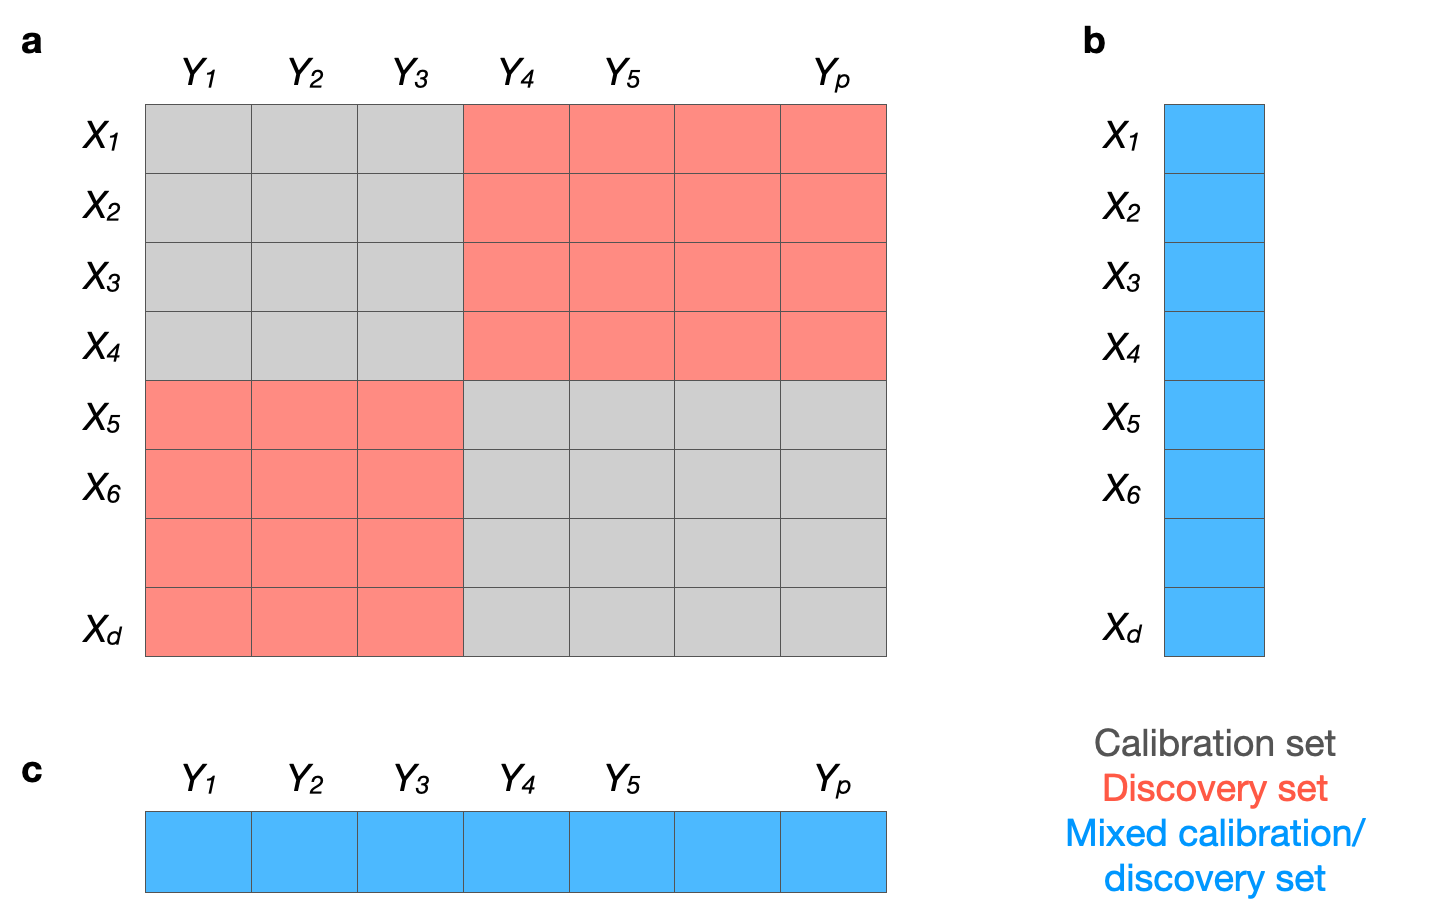
\includegraphics[width=1\linewidth]{calibration_sets}
	\caption{Comparison of three different types of data: (a) tall and wide, (b) tall, and (c) wide. Examples of (a) include eQTL, multimodal single-cell, and single-cell CRISPR screen data; an example of (b) is GWAS data; and examples of (c) include microarray and bulk RNA-seq data.}
	\label{fig:calibration_sets}
\end{figure}	

We argue that the shift from single-axis to multi-axis high-throughput data is a significant one. In particular, the shift opens the door to new ways of thinking about calibration. On single-axis high-throughput data, the ``calibration'' and ``discovery'' sets coincide: we must use the same data to test for associations and assess calibration. Traditionally, statisticians have relied on sparsity assumptions for this purpose. By contrast, on multi-axis high-throughput data, we can construct distinct calibration and discovery sets. This enables us to take a prediction-inspired approach to testing. Single-cell CRISPR screens, a new kind of genomic data rapidly gaining importance, typically come equipped with \textit{experimental} negative \textit{and} positive controls.

\section{A framework for negative controls}
Our goal is to formalize and unify the use of negative controls in conditional independence testing. Here, we consider the simplest, nontrivial case.
\textbf{Background}. As a review, suppose we seek to test the hypothesis $X \indep Y | Z$ using data $\{ (X_1, Y_1, Z_1)$, $\dots,$ $(X_n, Y_n, Z_n) \}$. Let $f_{X,Y,Z}$ be the joint density of $(X_i,Y_i,Z_i).$ The null hypothesis is true if and only if
$$ f_{X,Y|Z} = f_{Y|Z} f_{X|Z}$$ for some densities $f_{Y|Z}$, and $f_{X|Z}$. The null hypothesis, of course, is composite. Let $f^\textrm{null}_{X,Y|Z}$ be the set of densities that factors in the above manner. Next, let $\phi : (\R \times \R \times \R^d)^n \to \{0, 1\}$ be a test of the null hypothesis. We say that $\phi$ is level $\alpha$ if
$$ \sup_{ f \in f^\textrm{null}_{X,Y|Z}} \E_{f} \left[  \phi \left( \{ (X_i, Y_i, Z_i) \}_{i=1}^n \right)  \right]  \leq \alpha.$$

\noindent
\textbf{Statistical framework}. We now put ourselves in the ``high-multiplicity'' setting. Throughout, we condition on $Z$. Let $\{f^1_{X,Y|Z}, \dots f^p_{X,Y|Z}\}$ be $p$ conditional densities. Let $\{ D_1, \dots, D_p \}$ be $p$ independent (conditional on $Z$) datasets, where
$$D_i = \{ (X^i_1, Y^i_1, Z_1), \dots, (X^i_n, Y^i_n, Z_n) \},$$ and $$(X^i_1, Y^i_1), \dots, (X^i_n, Y^i_n) \sim f^i_{X, Y|Z}.$$ In other words, $D_i \in \R^{n \times (2 + d)}$ is a dataset consisting of the columns $X^i := (X^i_1, \dots, X^i_n),$ $Y^i := (Y^i_1, \dots, Y^i_n),$ and $Z := (Z_1, \dots, Z_n);$ the rows $\{ (X^i_j, Y^i_j) \}_{j=1}^n$ of the first two columns of $D_i$ are drawn i.i.d.\ from the conditional distribution $f^i_{X,Y|Z}$; and the final column $Z = (Z_1, \dots, Z_n)$ of $D_i$ is held constant across datasets.

For $i \in \{1, \dots, p\},$ let $H_i$ be the hypothesis that $$ f^i_{X,Y|Z} = f^i_{X|Z} f^i_{Y|Z}$$ for some $f^i_{X|Z}$ and $f^i_{Y|Z}.$ In other words, $H_i$ is the hypothesis that the conditional independence property holds for the $i$th density. We test hypothesis $H_i$ by applying a conditional independence test to dataset $D_i.$  Let $\mathcal{N} \subset \{1, \dots, p\}$ be the set of hypotheses for which the null hypothesis is true, and let $|\mathcal{N}|$ denote the number of true null hypotheses.

In many applications the conditional densities $f_{X|Z}^i$ and $f_{Y|Z}^i$ are similar across the $i$s. For example, in a single-cell CRISPR screen experiment, $\{f^i_{Y|Z}\}_{i=1}^p$ are the gene expression densities (conditional on the technical factors). These densities are similar across features: aside from some gene-to-gene variability in mean expression level and dispersion, the gene expression densities are all sparse, discrete counts.

We can encode this similarity across features using a Bayesian approach. Let $\{f_{X|Z}(\theta_X) : \theta_X \in \R^{m_x} \}$ be a family of densities parameterized by $\theta_X \in R^{m_x}.$ Similarly, let $\{ f_{Y|Z}(\theta_Y) : \theta_Y \in \R^{m_y} \}$ be a family of densities parameterized by $\theta_Y \in \R^{m_y}.$ Next, let $G_x$ and $G_y$ be probability distributions. We assume the following hierarchical model:
$$ 
\begin{cases}
\theta_X^1, \dots, \theta_X^p \sim G_x \\
f^1_{X|Z} = f_{X|Z}(\theta_X^1), \dots, f^p_{X|Z} = f_{X|Z}(\theta_X^p)
\\ 
 \theta^1_Y, \dots, \theta_Y^p \sim G_y
 \\ 
 f^1_{Y|Z} = f_{Y|Z}(\theta_Y^1), \dots, f^p_{Y|Z} = f_{Y|Z}(\theta_Y^p).
\end{cases}
$$
Hence, for $i \in \mathcal{N},$ the density factors as 
$$ f_{X,Y|Z}^i = f^i_{X|Z} f^i_{Y|Z} = f_{X|Z}(\theta_X^i) f_{Y|Z}(\theta_Y^i).$$
\\
\noindent
\textbf{Negative controls}. Negative controls exploit the similarity across features to assess calibration. For $i \in \{1, \dots, p_\textrm{nc} \}$, let $\tilde{f}^i_{X,Y|Z}$ denote the density of the $i$th negative control. By definition, the null hypothesis holds true for the negative controls, and so 
$$\tilde{f}^i_{X,Y|Z} = \tilde{f}^i_{X|Z} \tilde{f}^i_{Y|Z}$$ for some densities $\tilde{f}^i_{X|Z}$ and $\tilde{f}^i_{Y|Z}.$ Let $\tilde{D}_i \in \R^{2 + d}$ denote the dataset generated by $\tilde{f}^i_{X,Y|Z},$ i.e.
$$ \tilde{D}_i = \{ (\tilde{X}^i_1, \tilde{Y}^i_1, Z_1), \dots, (\tilde{X}^i_n, \tilde{Y}^i_n, Z_n)\},$$ where $$ (\tilde{X}^i_1, \tilde{Y}^i_1), \dots, (\tilde{X}^i_n, \tilde{Y}^i_n) \sim \tilde{f}^i_{X,Y|Z},$$ and $Z$ is the same as before. Our core assumption is that the negative control datasets are ``similar'' to the null datasets, which we formalize below.
\\ \\
\textit{\textbf{Key assumption}: Let $\tilde{\theta}^1_X, \dots, \tilde{\theta}^{p_\textrm{nc}}_X \sim G_x$ and $\tilde{\theta}^1_Y, \dots, \tilde{\theta}_Y^{p_\textrm{nc}} \sim G_y.$ We assume that that $\tilde{f}^i_{X|Z} = f_{X|Z}( \tilde{\theta}^i_X ) $ and $\tilde{f}^i_{Y|Z} = f_{X|Z}(\tilde{ \theta}^i_Y).$}
\\ \\
In other words, we assume that the conditional densities $f_{X|Z}$ and $f_{Y|Z}$ are drawn i.i.d.\ from the \textit{same} underlying distribution on both the negative control data \textit{and} the null data. A key corollary results from the assumption.
\\ \\
\textit{\textbf{Key corollary}: The null data $\{ D_i : i \in \mathcal{N} \}$ and the negative control data $\{ \tilde{D}_i \}_{i=1}^{p_\textrm{nc}}$ are identically distributed.}
\\ \\
This corollary implies that we can use the negative control data to assess calibration of the method on the rest of the data. To flesh this idea out, let $\phi_\alpha: ( \R \times \R \times \R^d )^n \to \{0,1\}$ be a level $\alpha$ test of the null hypothesis. If
$\E [ \phi_\alpha( \tilde{D}_i ) ] \leq \alpha$ (i.e., $\phi_\alpha$ controls type-I error at level $\alpha$ on the negative control data), it follows that $\E[ \phi_\alpha(D_i)]$ for $i \in \mathcal{N}$ (i.e., $\phi_\alpha$ controls type-I error on the null data). This is because $\tilde{D}_j \stackrel{d}{=} D_i$ for $i \in \mathcal{N}.$ Pulling back, in using negative controls, we implicitly make the assumption that the negative control datasets have a similar (or identical) distribution to the null datasets. The framework presented here is one way of formalizing that assumption.

%\\ \\
% \textbf{A more general array framework}. Above, we presented a framework for negative controls based on a toy model. In the context of single-cell CRISPR screens, we assumed that the number of negative control genes equaled the number of negative control gRNAs (namely, $p_\textrm{nc}$). We then constructed the negative control datasets by matching each negative control gene to a single negative control gRNA. 

% Ideas from prediction could be applied; for example, robustness to distribution shift, hyperparameter selection, cross validation, etc.


\section{An analogy between prediction and CI testing}

We propose a framework for CI testing with negative controls that is directly analogous to prediction. We propose the following steps:
\begin{itemize}
\item[1.] Let $\mathcal{S} = \{ D_1, \dots, D_B \}$ be the $B$ (possibly dependent) negative control datasets.
\item[2.] Partition the negative control datasets into train and validation sets in such a way that the two sets are independent (given $Z$). In other words, define sets $\mathcal{T}$ and $\mathcal{V}$ such that 
\begin{itemize}
\item[i.] $\mathcal{T} \cap \mathcal{V} = \emptyset.$
\item[ii.] $ \mathcal{T} \cup \mathcal{V} = \mathcal{S}.$ 
\item[iii.] $\mathcal{T} \indep \mathcal{V}.$
\end{itemize}
\end{itemize}

\begin{tabular}{|p{3cm}|p{5cm}|p{5cm}|}
	\hline 
 	 & Prediction & CI testing \\
 	 \hline 
 	Basic unit & An example $(X_i, Y_i, Z_i)$  & A negative control dataset $D_{ij} = \{ (X^i_l, Y^j_l, Z_l) \}_{l=1}^n$  \\ 
	\hline 
	 Algorithm & A CI test $\phi$ & A prediction function $f$  \\ 
	\hline 
	Ground truth & Label $Y_i$ available & Dataset $D_{ij}$ a negative control \\ 
	\hline 
	Calibration set & Subset of (known ground truth) data on which we train predictor & Subset of (known ground truth) data on which we calibrate CI testing method \\ 
	\hline 
	Validation set &  Subset of (known ground truth) data on which we assess predictor performance &  Subset of (known ground truth) data on which we assess CI method performance \\ 
	\hline 
	Discovery set & Unlabeled data $\{(X_i, Z_i)\}$ on which we seek prediction  & New data $\{ (X^i_l, Y^j_l, Z_l) \}_{l=1}^n$ with unknown ground truth \\ 
	\hline 
	Target metric & Type-I error as a function of $\alpha$, $E(\alpha)$: $$ E(\alpha) = \P( \phi(D_i) \leq \alpha ) $$ & Prediction risk $R$ given metric $d$: $$ R = \E[ d(Y_i, f(X_i, Z_i)) ] $$ \\ 
	\hline 
	Empirical metric & Empirical type-I error  & Empirical risk \\ 
	\hline 
\end{tabular} 

\section{Positive controls and partially synthetic positive controls}

We can use positive controls (real or semi-synthetic) to boost power in the calibration phase.

\section{Borrowing ideas from prediction}

The analogy enables us to borrow potentially useful ideas from prediction:
\begin{itemize}
\item Robustness to distribution shift
\item Hyperparameter tuning
\item Cross validation
\end{itemize}

\bibliographystyle{unsrt}
\bibliography{/Users/timbarry/Documents/optionFiles/library.bib}

\end{document}
